\documentclass[a4paper, 12pt, reqno]{amsart}

\usepackage{amssymb}
\usepackage{amsfonts}
\numberwithin{equation}{section}
\usepackage[margin=1in]{geometry}
\usepackage[english]{babel}
\usepackage[colorlinks, pdftitle={Actuarial Mathematics Homework 5},
    pdfauthor={Moritz M. Konarski}]{hyperref}
\usepackage{enumitem}
\usepackage{graphicx}
\usepackage{tikz}
\usetikzlibrary{snakes}
\renewcommand{\baselinestretch}{1.25}

\title{Actuarial Mathematics Homework 5}
\author{Moritz M. Konarski}
\date{\today}

\begin{document}

\maketitle

\section{Parmenter Exercises 2--11 to 2--19}

\subsection*{2--11}

Plan A:\\

\begin{center}
\begin{tikzpicture}
    \def\f{3}
    \draw (0,0) -- (\f*4,0);
    \foreach \x in {\f*1,\f*2,\f*3}
      \draw (\x cm,3pt) -- (\x cm,-3pt);
    \draw (\f*1,0) node[below=3pt, align=center] {$0$}
        node[above=3pt] {$150$};
    \draw (\f*2,0) node[below=3pt, align=center] {$1$}
        node[above=3pt] {$200$};
    \draw (\f*3,0) node[below=3pt, align=center] {$2$}
        node[above=3pt] {$250$};
\end{tikzpicture}
\end{center}

Plan B:\\

\begin{center}
\begin{tikzpicture}
    \def\f{3}
    \draw (0,0) -- (\f*4,0);
    \foreach \x in {\f*1,\f*2,\f*3}
      \draw (\x cm,3pt) -- (\x cm,-3pt);
    \draw (\f*1,0) node[below=3pt, align=center] {$0$}
        node[above=3pt] {$87$};
    \draw (\f*2,0) node[below=3pt, align=center] {$1$}
        node[above=3pt] {$425$};
    \draw (\f*3,0) node[below=3pt, align=center] {$2$}
        node[above=3pt] {$50$};
\end{tikzpicture}
\end{center}

Find the $i$ for which plan A is better than plan B for the consumer.
\begin{equation}\nonumber
        150(1+i)^2 + 200(1+i) + 250 < 87(1+i)^2 + 425(1+i) + 50
\end{equation}

Find the intersections and then check which plan is better in the interval
\begin{equation}\nonumber
    \begin{aligned}
        150(1+i)^2 + 200(1+i) + 250 &< 87(1+i)^2 + 425(1+i) + 50    \\
        1+i &= c\\
        0 = 63c^2 - &225c + 200 \\
        c_1 = \frac{40}{21} &\qquad c_2 = \frac{5}{3}   \\
        i_1 = \frac{19}{21} &\qquad i_2 = \frac{2}{3}
    \end{aligned}
\end{equation}

For $\frac{2}{3} < i < \frac{19}{21}$ plan A is better than plan B.

\subsection*{2--12}

Draw a timeline:\\

\begin{center}
\begin{tikzpicture}
    \def\f{2.5}
    \draw (0,0) -- (\f*5,0);
    \foreach \x in {\f*1,\f*2,\f*3,\f*4}
      \draw (\x cm,3pt) -- (\x cm,-3pt);
    \draw (\f*1,0) node[below=3pt, align=center] {$0$}
        node[above=3pt] {$300$};
    \draw (\f*2,0) node[below=3pt, align=center] {$1$}
        node[above=3pt] {$200$};
    \draw (\f*3,0) node[below=3pt, align=center] {$2$}
        node[above=3pt] {$100$};
    \draw (\f*4,0) node[below=3pt, align=center] {$3$}
        node[above=3pt] {$=800$};
\end{tikzpicture}
\end{center}

For which $i$ do the payments equal 800?
\begin{equation}\nonumber
    \begin{aligned}
        800 &= 300(1+i)^3 + 200(1+i)^2 + 100(1+i)   \\
        1 + i &= 1.12926    \\
        i &= 0.12926
    \end{aligned}
\end{equation}

\subsection*{2--13}

Draw a timeline:\\

\begin{center}
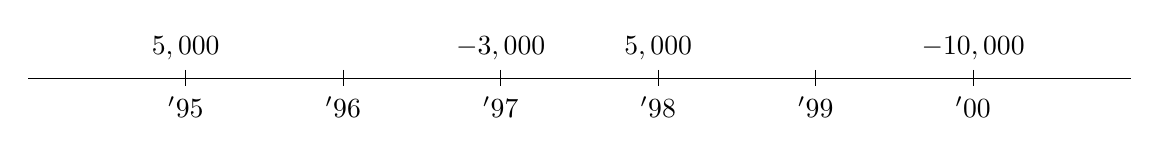
\begin{tikzpicture}
    \def\f{2}
    \draw (0,0) -- (\f*7,0);
    \foreach \x in {\f*1,\f*2,\f*3,\f*4,\f*5,\f*6}
      \draw (\x cm,3pt) -- (\x cm,-3pt);
    \draw (\f*1,0) node[below=3pt, align=center] {$'95$}
        node[above=3pt] {$5,000$};
    \draw (\f*2,0) node[below=3pt, align=center] {$'96$}
        node[above=3pt] {$ $};
    \draw (\f*3,0) node[below=3pt, align=center] {$'97$}
        node[above=3pt] {$-3,000$};
    \draw (\f*4,0) node[below=3pt, align=center] {$'98$}
        node[above=3pt] {$5,000$};
    \draw (\f*5,0) node[below=3pt, align=center] {$'99$}
        node[above=3pt] {$ $};
    \draw (\f*6,0) node[below=3pt, align=center] {$'00$}
        node[above=3pt] {$-10,000$};
\end{tikzpicture}
\end{center}

For which $i$ do the payments equal 0?
\begin{equation}\nonumber
    \begin{aligned}
        0 &= 5,000(1+i)^5 - 3,000(1+i)^3 + 5,000(1+i)^2 - 10,000 \\
        1 + i &= 1.097 \\
        i &= 0.097
    \end{aligned}
\end{equation}

\subsection*{2--14}

Draw a timeline:\\

\begin{center}
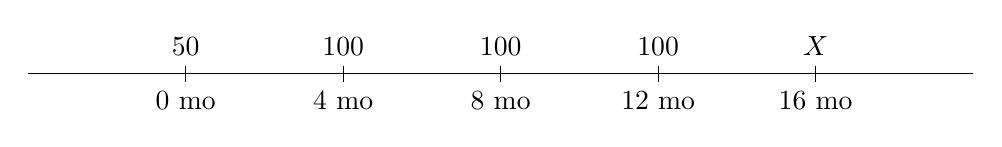
\begin{tikzpicture}
    \def\f{2}
    \draw (0,0) -- (\f*6,0);
    \foreach \x in {\f*1,\f*2,\f*3,\f*4,\f*5}
      \draw (\x cm,3pt) -- (\x cm,-3pt);
    \draw (\f*1,0) node[below=3pt, align=center] {$0$ mo}
        node[above=3pt] {$50$};
    \draw (\f*2,0) node[below=3pt, align=center] {$4$ mo}
        node[above=3pt] {$100$};
    \draw (\f*3,0) node[below=3pt, align=center] {$8$ mo}
        node[above=3pt] {$100$};
    \draw (\f*4,0) node[below=3pt, align=center] {$12$ mo}
        node[above=3pt] {$100$};
    \draw (\f*5,0) node[below=3pt, align=center] {$16$ mo}
        node[above=3pt] {$X$};
\end{tikzpicture}
\end{center}

\begin{enumerate}[label=(\alph*)]
    \item What is $X$ if $i=0.12$?
        \begin{equation}\nonumber
            \begin{aligned}
                i^{(4)} &= 4\left(\sqrt[4]{1+0.12}-1\right) = 0.11495    \\
                600 &= 50\left(1+i^{(4)}\right)^4 + 100\left(1+i^{(4)}\right)^3 
                    + 100\left(1+i^{(4)}\right)^2 + 100\left(1+i^{(4)}\right) + 
                    X \\
                X &= 148.32615
            \end{aligned}
        \end{equation}
    \item What is $i$ if $X=350$?
        \begin{equation}\nonumber
            \begin{aligned}
                600 = 50\left(1+i^{(4)}\right)^4 + 100\left(1+i^{(4)}\right)^3 
                    &+ 100\left(1+i^{(4)}\right)^2 + 100\left(1+i^{(4)}\right) + 
                    350 \\
                1 + i^{(4)} &= c \\
                c_1 = 0.85852   &\qquad c_2 = -2.06683  \\
                i_1^{(4)} = -0.13415 &\qquad i_2^{(4)} = -0.99703  
            \end{aligned}
        \end{equation}
\end{enumerate}

\subsection*{2--15}

7\% effective interest at the end of each year, every 4 years 5\% bonus on
existing money. Find the effective rate for 
\begin{enumerate}[label=(\alph*)]
    \item 3 years
        \begin{equation}\nonumber
            (1+0.07)^3 - 1 = 0.22504
        \end{equation}
    \item 4 years
        \begin{equation}\nonumber
            (1+0.07)^4 \cdot 1.05 - 1 = 0.37634
        \end{equation}
    \item 5 years
        \begin{equation}\nonumber
            (1+0.07)^5 \cdot 1.05 \cdot 1.07 - 1 = 0.47268
        \end{equation}
\end{enumerate}

\subsection*{2--16}

The sum of all payments of 1 every 3 years from 1 to $n$ while $n$ approaches
infinity is 
\begin{equation}\nonumber
    \lim_{n\rightarrow\infty} \left( 1 + 1 \cdot \left(1+i^{(m)}\right)
        + 1 \cdot \left(1+i^{(m)}\right)^3 + \dots
        + 1 \cdot \left(1+i^{(m)}\right)^n \right)
\end{equation}

And we know that the present value times the interest to the power of $n$
approaching infinity is this
\begin{equation}\nonumber
    \lim_{n\rightarrow\infty} \left( \frac{125}{91} 
        \cdot \left(1+i^{(m)}\right)^n \right)
\end{equation}

We can set these two equal
\begin{equation}\nonumber
    \begin{aligned}
        \lim_{n\rightarrow\infty} &\left(1 + 1 \cdot \left(1+i^{(m)}\right)
            + 1 \cdot \left(1+i^{(m)}\right)^3 + \dots
            + 1 \cdot \left(1+i^{(m)}\right)^n \right) \\
        &=\lim_{n\rightarrow\infty} \left(\frac{125}{91} \cdot \left(1+i^{(m)}
            \right)^n \right)
    \end{aligned}
\end{equation}

and divide both sides by $\left(1+i^{(m)}\right)^{n-1}$
\begin{equation}\nonumber
    \begin{aligned}
        \lim_{n\rightarrow\infty} &\left(1 \cdot
        \left(1+i^{(m)}\right)^{n-1} + 1 \cdot
        \left(1+i^{(m)}\right)^{n-2}
            + \dots  +  1
            + 1 \cdot \left(1+i^{(m)}\right) \right) \\
        &=\lim_{n\rightarrow\infty} \left(\frac{125}{91} \cdot \left(1+i^{(m)}
            \right) \right)
    \end{aligned}
\end{equation}

Taking the limit we get
\begin{equation}\nonumber
    1 + \left(1+i^{(m)}\right)
    =\frac{125}{91} \cdot \left(1+i^{(m)}\right)
\end{equation}

We find that 
\begin{equation}\nonumber
    i^{(m)} = \frac{1}{\frac{125}{91}-1} - 1
\end{equation}

and thus 
\begin{equation}\nonumber
    i = \left[ 1 + \frac{\frac{1}{\frac{125}{91}-1} - 1}{1/3} \right]^{1/3} - 1
        = 0.820085
\end{equation}

Testing the result for $n$ from 0 to 50,000, the results match relatively well.
The sum of individual payments is 8.506E+13004 and the present value function
gives 5.264E+13004.

\subsection*{2--17}

\begin{center}
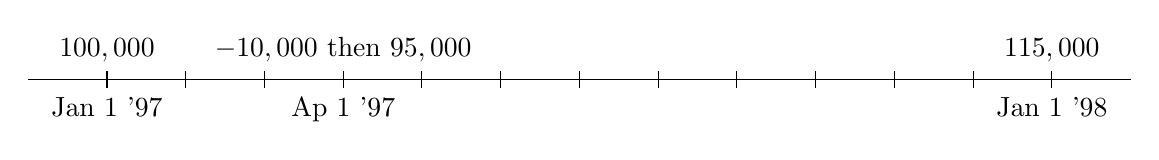
\begin{tikzpicture}
    \def\f{1}
    \draw (0,0) -- (\f*14,0);
    \foreach \x in
    {\f*1,\f*2,\f*3,\f*4,\f*5,\f*6,\f*7,\f*8,\f*9,\f*10,\f*11,\f*12,\f*13}
      \draw (\x cm,3pt) -- (\x cm,-3pt);
    \draw (\f*1,0) node[below=3pt, align=center] {Jan 1 '97}
        node[above=3pt] {$100,000$};
    \draw (\f*4,0) node[below=3pt, align=center] {Ap 1 '97}
        node[above=3pt] {$-10,000$ then $95,000$};
    \draw (\f*13,0) node[below=3pt, align=center] {Jan 1 '98}
        node[above=3pt] {$115,000$};
\end{tikzpicture}
\end{center}

\begin{enumerate}[label=(\alph*)]
    \item Find the time weighted interest
        \begin{equation}\nonumber
            \begin{aligned}
                i &= \frac{105,000}{100,000} \cdot \frac{115,000}{95,000} -1 \\
                i &= 0.27105
            \end{aligned}
        \end{equation}
    \item Find the simple interest rate for the year
        \begin{equation}\nonumber
            \begin{aligned}
                1 + i &= c  \\
                115,000 &= 100,000c^{12} - 10,000c^9    \\
                c_1 = 1.02009 &\qquad c_2 < 0       \\
                i^{(12)} &= 0.02009  \\
                i &= 0.26959
            \end{aligned}
        \end{equation}
    \item Find the simple interest rate for the year assuming equal spacing of
        payments
        \begin{center}
        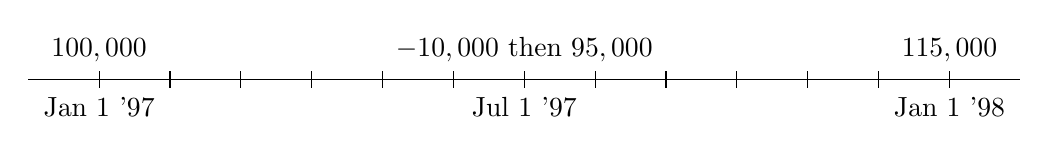
\begin{tikzpicture}
            \def\f{0.9}
            \draw (0,0) -- (\f*14,0);
            \foreach \x in
            {\f*1,\f*2,\f*3,\f*4,\f*5,\f*6,\f*7,\f*8,\f*9,\f*10,\f*11,\f*12,\f*13}
              \draw (\x cm,3pt) -- (\x cm,-3pt);
            \draw (\f*1,0) node[below=3pt, align=center] {Jan 1 '97}
                node[above=3pt] {$100,000$};
            \draw (\f*7,0) node[below=3pt, align=center] {Jul 1 '97}
                node[above=3pt] {$-10,000$ then $95,000$};
            \draw (\f*13,0) node[below=3pt, align=center] {Jan 1 '98}
                node[above=3pt] {$115,000$};
        \end{tikzpicture}
        \end{center}
        \begin{equation}\nonumber
            \begin{aligned}
                1 + i &= c  \\
                115,000 &= 100,000c^{2} - 10,000c    \\
                c_1 = 1.12354 &\qquad c_2 < 0       \\
                i^{(2)} &= 0.12354  \\
                i &= 0.26234
            \end{aligned}
        \end{equation}
\end{enumerate}

\subsection*{2--18}

\begin{center}
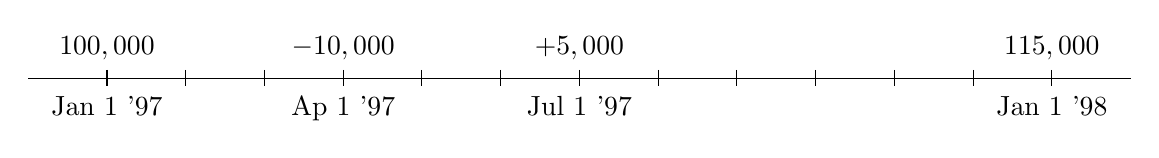
\begin{tikzpicture}
    \def\f{1}
    \draw (0,0) -- (\f*14,0);
    \foreach \x in
    {\f*1,\f*2,\f*3,\f*4,\f*5,\f*6,\f*7,\f*8,\f*9,\f*10,\f*11,\f*12,\f*13}
      \draw (\x cm,3pt) -- (\x cm,-3pt);
    \draw (\f*1,0) node[below=3pt, align=center] {Jan 1 '97}
        node[above=3pt] {$100,000$};
    \draw (\f*4,0) node[below=3pt, align=center] {Ap 1 '97}
        node[above=3pt] {$-10,000$};
    \draw (\f*7,0) node[below=3pt, align=center] {Jul 1 '97}
        node[above=3pt] {$+5,000$};
    \draw (\f*13,0) node[below=3pt, align=center] {Jan 1 '98}
        node[above=3pt] {$115,000$};
\end{tikzpicture}
\end{center}

\begin{enumerate}[label=(\alph*)]
    \item Find the simple interest rate for the year
        \begin{equation}\nonumber
            \begin{aligned}
                1 + i &= c  \\
                115,000 &= 100,000c^{4} - 10,000c^3 + 5,000c^2    \\
                c_1 = 1.04889 &\qquad c_2,c_3,c_4 \text{ are negative or
                    complex}      \\
                i^{(4)} &= 0.04889  \\
                i &= 0.21037
            \end{aligned}
        \end{equation}
    \item Find the simple interest rate for the year assuming equal spacing of
        payments
        \begin{center}
        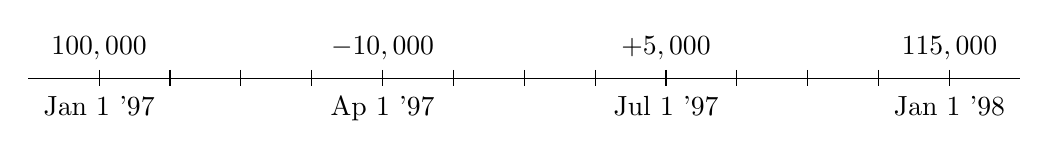
\begin{tikzpicture}
            \def\f{0.9}
            \draw (0,0) -- (\f*14,0);
            \foreach \x in
            {\f*1,\f*2,\f*3,\f*4,\f*5,\f*6,\f*7,\f*8,\f*9,\f*10,\f*11,\f*12,\f*13}
              \draw (\x cm,3pt) -- (\x cm,-3pt);
            \draw (\f*1,0) node[below=3pt, align=center] {Jan 1 '97}
                node[above=3pt] {$100,000$};
            \draw (\f*5,0) node[below=3pt, align=center] {Ap 1 '97}
                node[above=3pt] {$-10,000$};
            \draw (\f*9,0) node[below=3pt, align=center] {Jul 1 '97}
                node[above=3pt] {$+5,000$};
            \draw (\f*13,0) node[below=3pt, align=center] {Jan 1 '98}
                node[above=3pt] {$115,000$};
        \end{tikzpicture}
        \end{center}
        \begin{equation}\nonumber
            \begin{aligned}
                1 + i &= c  \\
                115,000 &= 100,000c^{3} - 10,000c^2 + 5,000c    \\
                c_1 = 1.06569 &\qquad c_2,c_3 < 0       \\
                i^{(3)} &= 0.0.6569 \\
                i &= 0.210299
            \end{aligned}
        \end{equation}
    \item You cannot find the time weighted interest because we don't know the
        value immediately before or after the deposit of 5,000.
\end{enumerate}

\subsection*{2--19}

\begin{center}
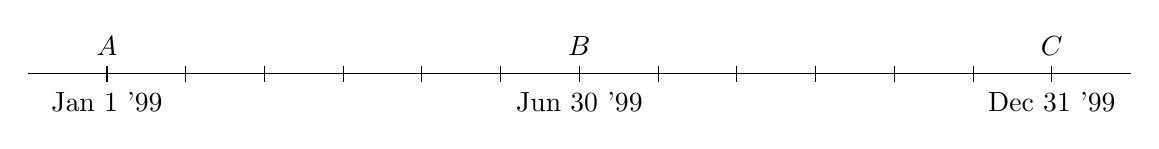
\begin{tikzpicture}
    \def\f{1}
    \draw (0,0) -- (\f*14,0);
    \foreach \x in
    {\f*1,\f*2,\f*3,\f*4,\f*5,\f*6,\f*7,\f*8,\f*9,\f*10,\f*11,\f*12,\f*13}
      \draw (\x cm,3pt) -- (\x cm,-3pt);
    \draw (\f*1,0) node[below=3pt, align=center] {Jan 1 '99}
        node[above=3pt] {$A$};
    \draw (\f*7,0) node[below=3pt, align=center] {Jun 30 '99}
        node[above=3pt] {$B$};
    \draw (\f*13,0) node[below=3pt, align=center] {Dec 31 '99}
        node[above=3pt] {$C$};
\end{tikzpicture}
\end{center}

\begin{enumerate}[label=(\alph*)]
    \item Find the time weighted interest
        \begin{equation}\nonumber
            i = \frac{B-A}{A} \cdot \frac{C-B}{B}
        \end{equation}
        and the simple interest
        \begin{equation}\nonumber
            i = \frac{C}{A}
        \end{equation}
    \item Find the simple and time weighted interest rate for a deposit $W$
        immediately after $B$
        \begin{center}
        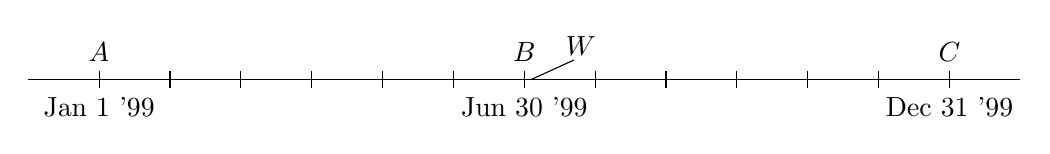
\begin{tikzpicture}
            \def\f{0.9}
            \draw (0,0) -- (\f*14,0);
            \foreach \x in
            {\f*1,\f*2,\f*3,\f*4,\f*5,\f*6,\f*7,\f*8,\f*9,\f*10,\f*11,\f*12,\f*13}
              \draw (\x cm,3pt) -- (\x cm,-3pt);
            \draw (\f*1,0) node[below=3pt, align=center] {Jan 1 '99}
                node[above=3pt] {$A$};
            \draw (\f*7,0) node[below=3pt, align=center] {Jun 30 '99}
                node[above=3pt] {$B$};
            \draw (\f*7.7 cm,7pt) -- (\f*7.1 cm,0);
            \draw (\f*7.8,0) node[below=3pt, align=center] {$ $}
                node[above=5pt] {$W$};
            \draw (\f*13,0) node[below=3pt, align=center] {Dec 31 '99}
                node[above=3pt] {$C$};
        \end{tikzpicture}
        \end{center}
        Time weighted interest
        \begin{equation}\nonumber
            i = \frac{B-A}{A} \cdot \frac{C-B+W}{B-W} 
                = \left(\frac{B}{A} -1 \right)\left(\frac{C}{B-W} +1  \right)
        \end{equation}
        Simple interest
        \begin{equation}\nonumber
            i_{1,2}^{(2)} = \frac{-W \pm \sqrt{W^2+4AC}}{2A} -1
        \end{equation}
    \item Find the simple and time weighted interest rate for a deposit $W$
        immediately before $B$
        \begin{center}
        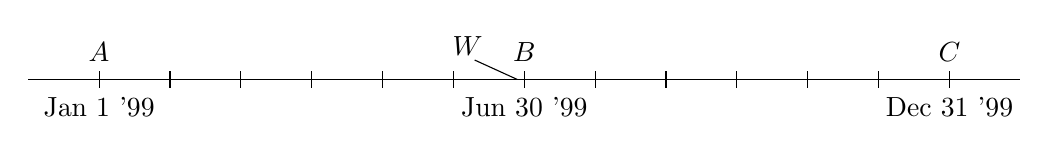
\begin{tikzpicture}
            \def\f{0.9}
            \draw (0,0) -- (\f*14,0);
            \foreach \x in
            {\f*1,\f*2,\f*3,\f*4,\f*5,\f*6,\f*7,\f*8,\f*9,\f*10,\f*11,\f*12,\f*13}
              \draw (\x cm,3pt) -- (\x cm,-3pt);
            \draw (\f*1,0) node[below=3pt, align=center] {Jan 1 '99}
                node[above=3pt] {$A$};
            \draw (\f*7,0) node[below=3pt, align=center] {Jun 30 '99}
                node[above=3pt] {$B$};
            \draw (\f*6.3 cm,7pt) -- (\f*6.9 cm,0);
            \draw (\f*6.2,0) node[below=3pt, align=center] {$ $}
                node[above=5pt] {$W$};
            \draw (\f*13,0) node[below=3pt, align=center] {Dec 31 '99}
                node[above=3pt] {$C$};
        \end{tikzpicture}
        \end{center}
        Time weighted interest
        \begin{equation}\nonumber
            i = \frac{B-A-W}{A} \cdot \frac{C-B}{B} 
                = \left(\frac{B-W}{A} -1 \right)\left(\frac{C}{B} -1  \right)
        \end{equation}
        Simple interest
        \begin{equation}\nonumber
            i_{1,2}^{(2)} = \frac{-W \pm \sqrt{W^2+4AC}}{2A} -1
        \end{equation}
    \item The simple rates of interest in (b) and (c) are identical because for
        simple interest it does not matter when a deposit happens relative to
        a known account balance as long as the deposit still happens at the
        same time (which it does).
    \item Show that if $W$ is a deposit ($W>0$), the time weighted interest in
        (b) is greater than the one in (c)
        \begin{equation}\nonumber
            \left(\frac{B-W}{A} -1 \right)\left(\frac{C}{B} -1  \right)
            < \left(\frac{B}{A}-1\right)\left(\frac{C}{B-W}+1\right)
        \end{equation}
        Comparing one factor from each side we see that
        \begin{equation}\nonumber
            \frac{B-W}{A} -1 < \frac{B}{A}-1
        \end{equation}
        because $B-W < B$. Examining the second pair of factors we see
        \begin{equation}\nonumber
            \frac{C}{B} -1 < \frac{C}{B-W}+1
        \end{equation}
        because again $B-W < B$. Thus we may conclude that
        \begin{equation}\nonumber
            \left(\frac{B-W}{A} -1 \right)\left(\frac{C}{B} -1  \right)
            < \left(\frac{B}{A}-1\right)\left(\frac{C}{B-W}+1\right)
        \end{equation}
\end{enumerate}

\end{document}
